
\setcounter{chapter}{3}
\chapter{Sprint 2: User and App Managment}
\minitoc %insert la minitoc
\graphicspath{{Chapter4/figures/}}

%\DoPToC
%==============================================================================
\pagestyle{fancy}
\fancyhf{}
\fancyhead[R]{\bfseries\rightmark}
\fancyfoot[R]{\thepage}
\renewcommand{\headrulewidth}{0.5pt}
\renewcommand{\footrulewidth}{0pt}
\renewcommand{\chaptermark}[1]{\markboth{\MakeUppercase{\chaptername~\thechapter. #1 }}{}}
\renewcommand{\sectionmark}[1]{\markright{\thechapter.\thesection~ #1}}

\begin{spacing}{1.2}

%==============================================================================
\section*{Introduction}
In order to integrate Flouci as a web payment method, we opted for an app model. This model consists of creating an app for each integration the developer wants to have. Each app contains basic information about the e-commerce website and is linked to a Flouci account to accept payment directly.
\newline
In this chapter, we will start our project development. We will focus on implementing two linked parts of our application which are the user and app.

\section{Flux Design Pattern}
Our solution is implemented with two main frameworks, Spring Boot and React JS.
Our back-end is entirely written with Spring Boot and serves as an API for our front-end developed with React.
\newline

Using React JS we had to follow a newly created design pattern called Flux. The pattern was created by Facebook and they define it as follows :
\newline

\say{Flux \cite{Flux} is the application architecture that Facebook uses for building client-side web applications. It complements React's composable view components by utilizing a unidirectional data flow. It's more of a pattern rather than a formal framework, and you can start using Flux immediately without a lot of new code.}

\begin{figure}[H]\centering
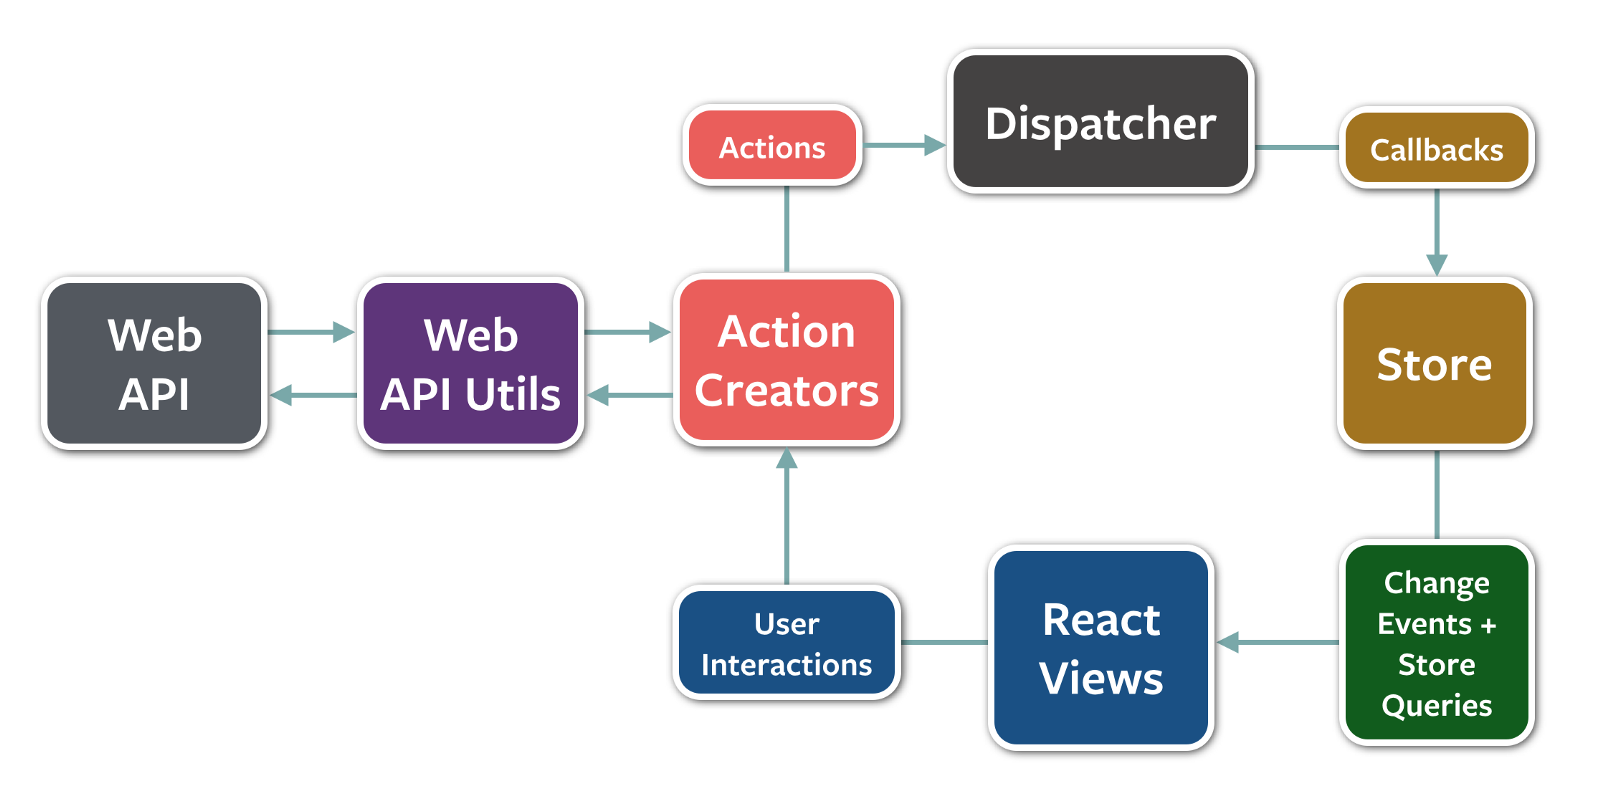
\includegraphics[scale=0.3]{Fluxdesignpattern.png}
\caption{Flux Design Pattern}
\label{usermanagementusecase}
\end{figure}

Flux is made up of 4 key elements:

\begin{itemize}
	\item \textbf{Actions:} Objects with property and data.
	\item \textbf{Stores:} Contain the application's state and logic.
	\item \textbf{The Dispatcher:} Processes registered actions and callbacks.
	\item \textbf{Views:} Listen to changes from the stores and re-render themselves.
\end{itemize}

\section{Sprint Use Cases}
In this section, we will start by understanding the Sprint specification by looking into the use cases diagrams.

\subsection{User Management Use Case}
Each project starts with the user management section. This section is about the basic user management features.

The figure \ref{usermanagementusecase} shows the user management use case diagram.
\begin{figure}[H]\centering
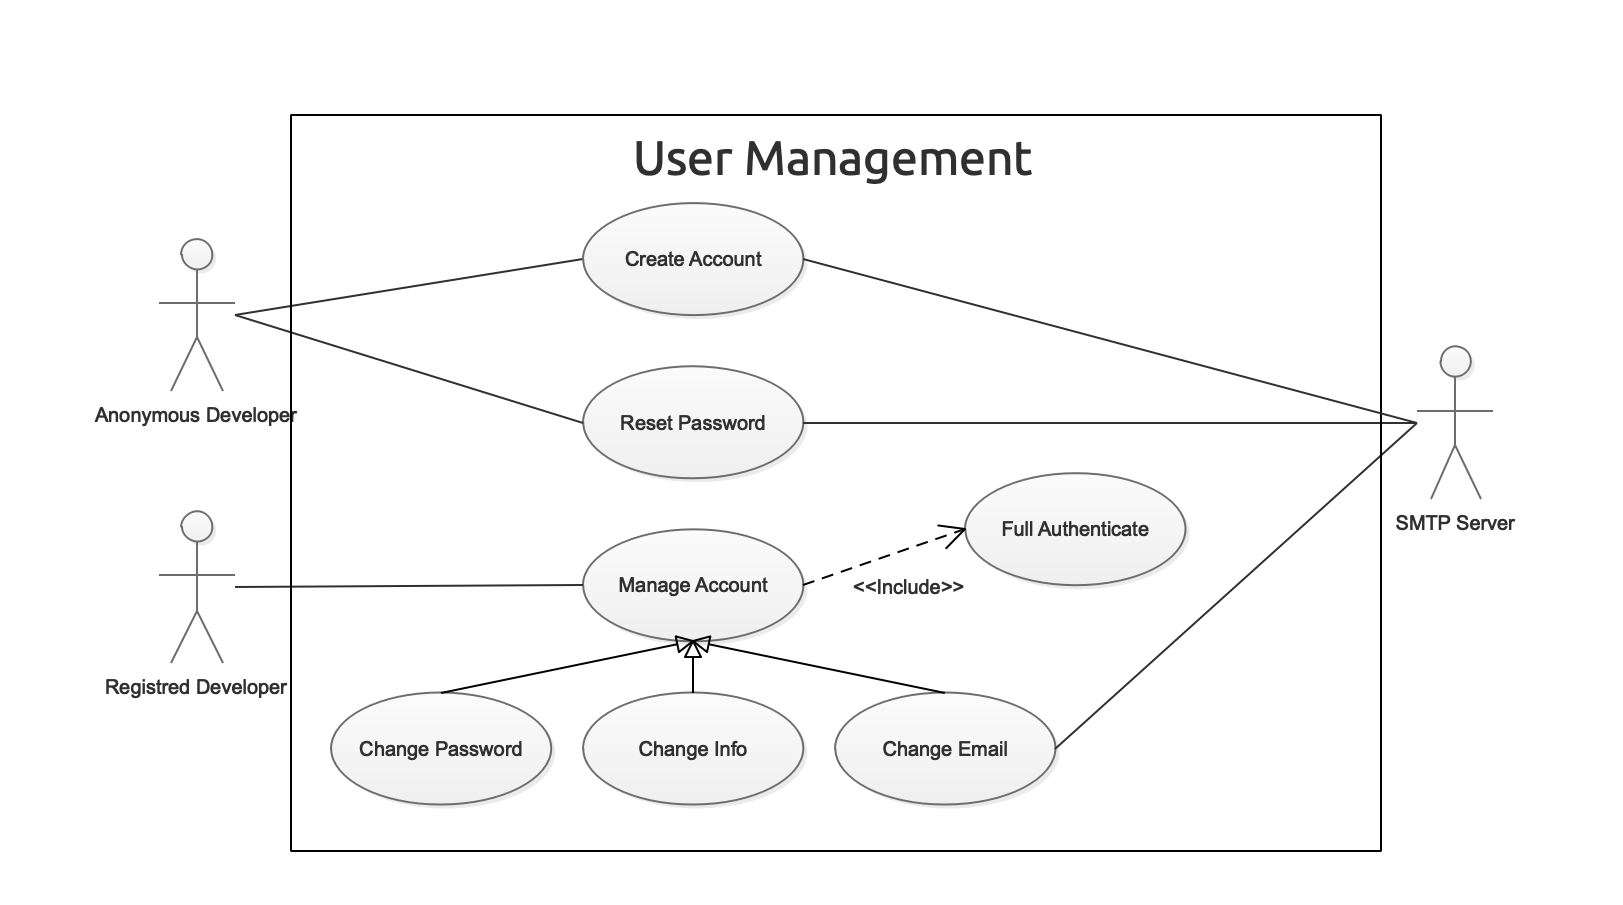
\includegraphics[scale=0.3]{userusecase.png}
\caption{User Management Use Case Diagram}
\label{usermanagementusecase}
\end{figure}


\subsection{App Management Use Case}
For every integration, the developer should create an integration app.
The app is linked to a Flouci wallet, and it contains two keys: public and private.
The keys are used in the process of integrating the app on e-commerce websites.


The figure \ref{appmanagementusecase} shows the use case diagram, and the table \ref{apptable} is a textual description of the main use case "create app".
\begin{figure}[H]\centering
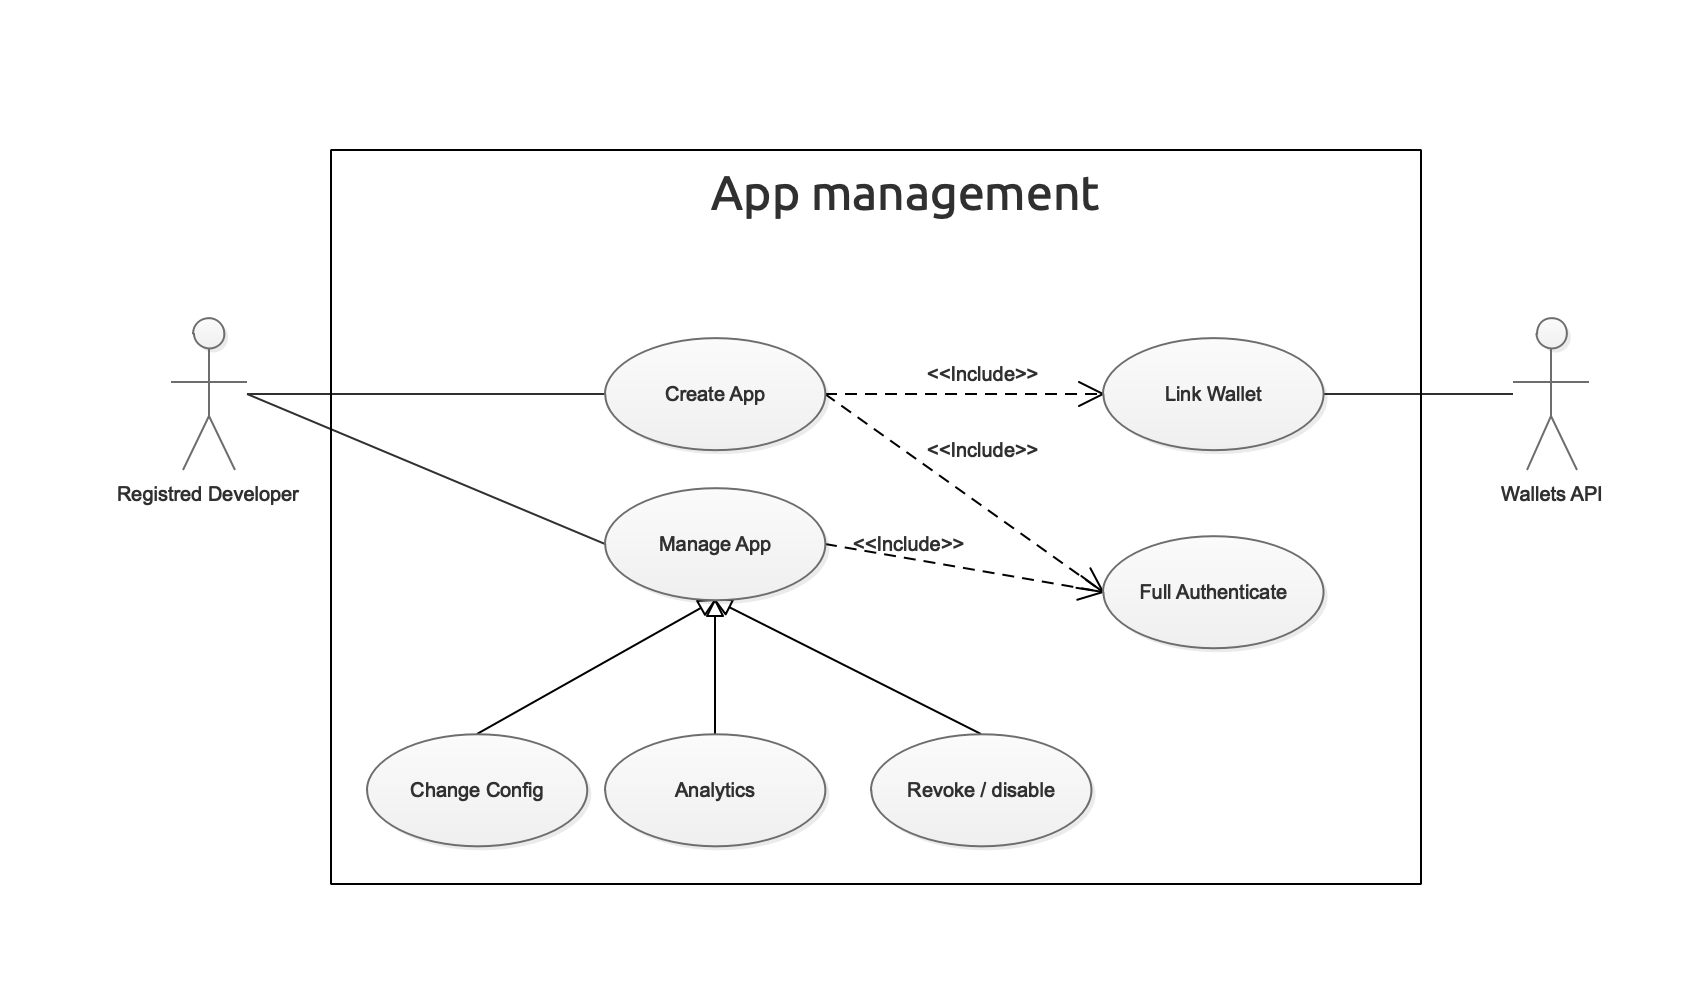
\includegraphics[scale=0.3]{appusecase.png}
\caption{App Management Use Case Diagram}
\label{appmanagementusecase}
\end{figure}

\begin{table}[H]
\centering
\caption{Text description of the create app use case}
\begin{tabularx}{\linewidth}{|c|X|}
\hline
Title & Create app.  \\ \hline
Summary & The user creates an integration app to use it on his e-commerce website. \\ \hline
Actors & Registered developer. \\ \hline
Precondition & The user visits the new app page. \\ \hline
Nominal Scenario & \begin{enumerate}
 \item The user enters the app name, description and a phone number linked to a Flouci wallet.
 \item The user gets an OTP on his phone number.
 \item The user enters the OTP to activate the app.
 \item The user is redirected to the newly created app page.
 \end{enumerate}
 \\ \hline
Alternative Scenarios & \begin{itemize}
	\item A1 If the app name is already used, the user should change the name.
	\item A2 If the phone number is not linked to a business wallet the user is asked to verify the number.
	\item A3 If the OTP is never received the user can ask to resend OTP.
	\item A3 If the user enters a wrong OTP he is asked to retry with a limit of three times.
\end{itemize} \\ \hline
Exceptional Scenario & If the user exceeds the maximum number of apps, he cannot create a new app. \\ \hline
Post-condition & The user is redirected to the app page. \\ \hline
\end{tabularx}
\label{apptable}
\end{table}

\section{Platform Design}
Before diving into writing the code, we started by modeling the platform using Adobe XD. This was very helpful for us since it made it possible to focus on the key features we want to have.

The Figure \ref{developersPlatform} represents the developer's API platform model we ended up with. It offers the same user experience of the other Kaoun products, including Flouci.

\begin{figure}[H]\centering
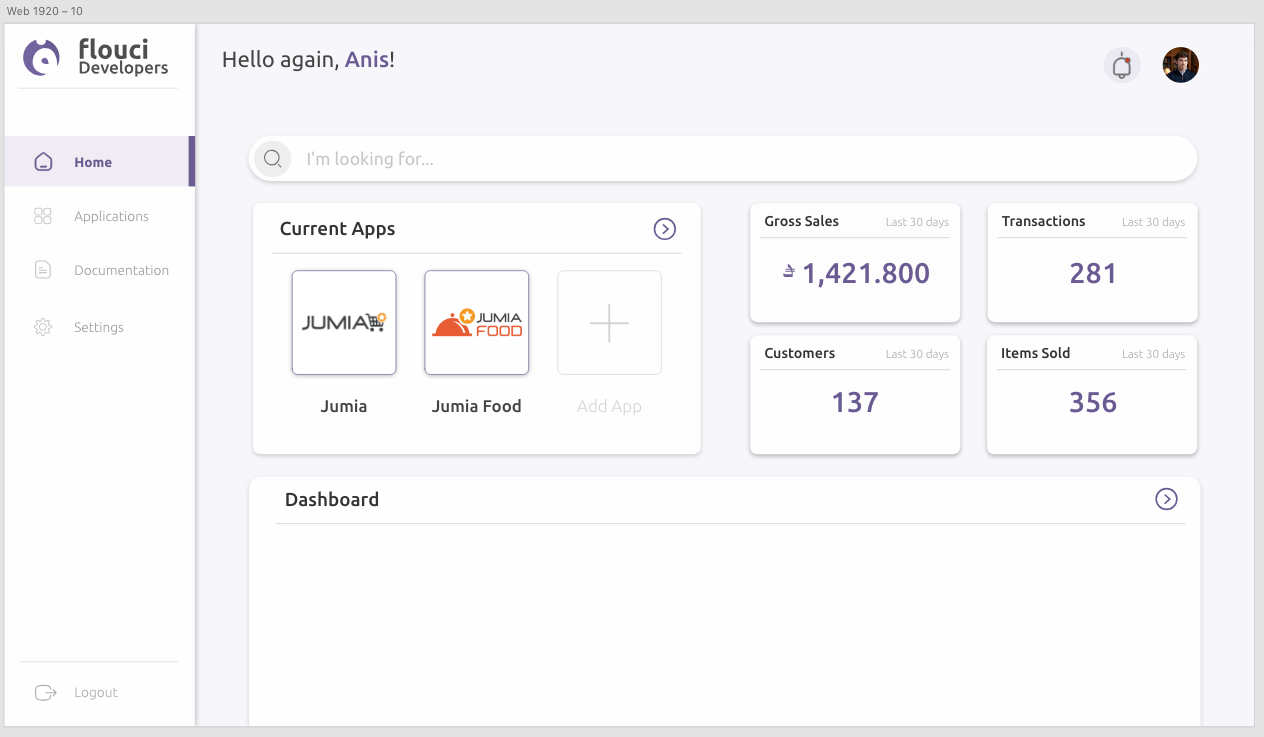
\includegraphics[scale=0.4]{web_screen}
\caption{Developers Platform Mock-up}
\label{developersPlatform}
\end{figure}

\section{User Management}
In this section we will explain our user management strategy, the mechanism of creating the account and the different authorities used. we also present how to recover a lost account.
\subsection{Authorities}
In our project we used four different authorities to manage access to different parts of the app:
\begin{itemize}
	\item \textbf{System}:  is mainly used by our audit logs, when something is done automatically
	\item \textbf{AnonymousUser:}  is given to anonymous users when they do an action
	\item \textbf{Developer}:  is a normal user with 'ROLE\_DEVELOPER' authorization it gives access to managing apps.
	\item  \textbf{Admin}:  is an admin user with 'ROLE\_DEVELOPER' and 'ROLE\_ADMIN' authorizations, he can manage users.
\end{itemize}

\subsection{Registration}
The registration process is very simple. We only require basic info and a valid email address to open an account. All created accounts have a "DEVELOPER" authorities which essentially give them access to restricted functionalities.

We only activate the user account after the email confirmation. The activation email contains a link with a key saved in the database. Accessing the link will activate the account.

The figure \ref{fig:register} is a sequence diagram that presents all the step needs to create a new account.

\begin{figure}[H]\centering
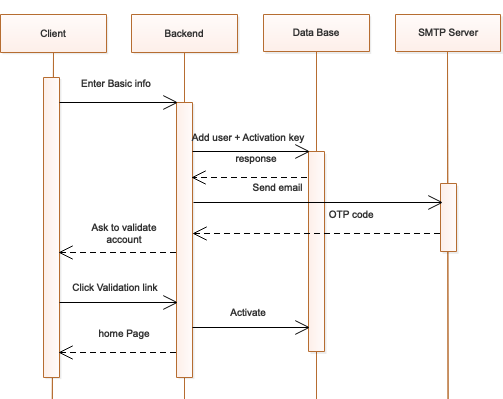
\includegraphics[scale=0.8]{Register_user_sequence_diagram.png}
\caption{User Registration Sequence Diagram}
\label{fig:register}
\end{figure}



\subsection{Recover Account}
In case the user forgets his password, he can simply reset it by email. We attach a key to the request and we send the URL with the key to the email. The link with the key takes the user to a page where he can change a new password. After that, our backend checks the reset key and apply the changes.

\section{App Management}
In our project, each e-commerce website is linked to an app to be able to accept Flouci as a payment method.
In this section, we will explain key functionalities of the app.
\subsection{App Creation}
Every app is linked to a Flouci Merchant account. Besides the basic information, the developer should enter a phone number to identify the Flouci account, then confirm it with the OTP key he gets by SMS.

After finishing creating the app, the developer will obtain two tokens.

The figure \ref{fig:appcreate} shows the whole process in detail.
\begin{figure}[H]\centering
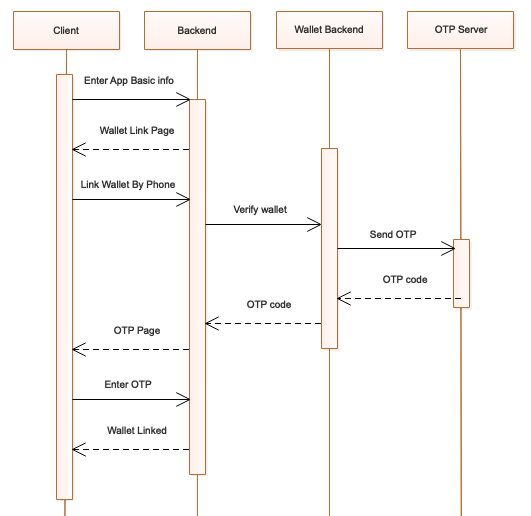
\includegraphics[width=\textwidth,height=12cm]{Create_App_Sequence_Diagram.png}
\caption{App creation Sequence Diagram}
\label{fig:appcreate}
\end{figure}
\subsection{App Revoke}
Since the app has two main tokens (public and private), we offer the possibility to revoke an app simply by changing its public token. Changing the token will result in obsoletion of all current integrations of the app, as they all will use a public token that doesn't resolve our app.

\subsection{App Metrics}
After the integration, there is a huge  risk of the developer shifting away from the platform. We decided to gather metrics for the user to be able to incentivize him to continue using to the platform.
Each app has two main metrics.
\begin{itemize}
	\item \textbf{Transactions:} the number of orders made.
	\item \textbf{Gross sales:} the total amount of all orders.
\end{itemize}
We also save the metrics per day with a cron job, so we can easily create charts to monitor sales.

\subsection{Orders}
With every online payment, we attach the app ID to the payment payload. This information will help us get the list of orders for each app.
We can then display all orders made, add filtering and even add a button to reimburse orders.

\section{Data Schema}
Our database model can be divided into three big sections of the projects. We have tables managing the user data, tables managing the app data and other independent tables handling auditing events. We have also made the model in a way that the user can have from 0 to N apps and an app can only be linked to one user.
The database schema is presented in the figure \ref{fig:database}
\begin{figure}[H]\centering
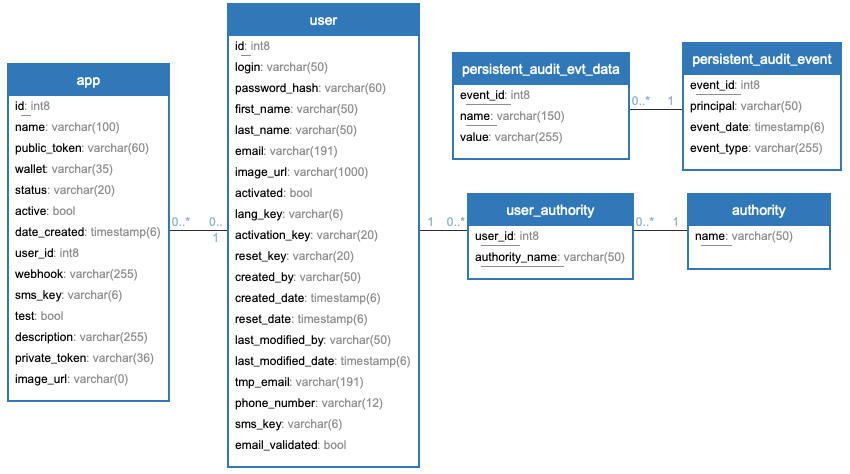
\includegraphics[width=\textwidth,keepaspectratio]{db.png}
\caption{Database Model}
\label{fig:database}
\end{figure}

\section*{Conclusion}
In this section, we implemented the first steps the user should do in order to integrate Flouci. After creating an account and an app, The two tokens provided will be the only missing piece to integrate Flouci payment method.

In the next section, we will implement the checkout API which can be integrated into any e-commerce website.
%==============================================================================
\end{spacing}
